\documentclass[twocolumn]{Styles/IEEEtran11}


\usepackage[usenames,dvipnames]{xcolor} % for colored text
\usepackage[normalem]{ulem} % for strikethrough text

% quantum macros

\def\01{\{0,1\}}
\def\eps{\epsilon}
\newcommand{\half}{{\frac{1}{2}}}
\newcommand{\set}[1]{{\left\{#1\right\}}}
\newcommand{\ksubsets}{{n \choose k}}
\newcommand{\jsubsets}{{n \choose j}}
\newcommand{\Prob}{{\mathbf{Pr}}}
\newcommand{\tinyspace}{\mspace{1mu}}
\newcommand{\microspace}{\mspace{0.5mu}}
\newcommand{\op}[1]{\operatorname{#1}}

\newcommand{\norm}[1]{\left\lVert\tinyspace#1\tinyspace\right\rVert}
\newcommand{\snorm}[1]{\lVert\tinyspace#1\tinyspace\rVert}
\newcommand{\abs}[1]{\left\lvert\tinyspace #1 \tinyspace\right\rvert}
\newcommand{\ceil}[1]{\left\lceil #1 \right\rceil}
\newcommand{\floor}[1]{\left\lfloor #1 \right\rfloor}
\def\iso{\cong}
\newcommand{\defeq}{\stackrel{\smash{\text{\tiny def}}}{=}}
\newcommand{\tr}{\operatorname{tr}}
\newcommand{\rank}{\operatorname{rank}}
\renewcommand{\det}{\operatorname{Det}}
\newcommand{\im}{\operatorname{Im}}
\renewcommand{\t}{{\scriptscriptstyle\mathsf{T}}}
\newcommand{\ip}[2]{\left\langle #1 , #2\right\rangle}
\newcommand{\ipp}[1]{\left\langle #1 \right\rangle}
\newcommand{\sip}[2]{\langle #1 | #2\rangle}

\def\({\left(}
\def\){\right)}
\def\I{\mathsf{id}}

\newcommand{\fid}{\operatorname{F}}
\newcommand{\setft}[1]{\mathrm{#1}}
\newcommand{\lin}[1]{\setft{L}\left(#1\right)}
\newcommand{\density}[1]{\setft{Dens}\left(#1\right)}
\newcommand{\unitary}[1]{\setft{U}\left(#1\right)}
\newcommand{\trans}[1]{\setft{T}\left(#1\right)}
\newcommand{\herm}[1]{\setft{Herm}\left(#1\right)}
\newcommand{\pos}[1]{\setft{Pos}\left(#1\right)}
\newcommand{\pd}[1]{\setft{Pd}\left(#1\right)}
\newcommand{\sphere}[1]{\mathcal{S}\!\left(#1\right)}
\newcommand{\opset}[3]{\setft{#1}_{#2}\!\left(#3\right)}
\newcommand{\ot}{\otimes}

\def\complex{\mathbb{C}}
\def\real{\mathbb{R}}
\def\natural{\mathbb{N}}
\def\integer{\mathbb{Z}}

\def\<{\langle}
\def\>{\rangle}
\def \lket {\left|}
\def \rket {\right\rangle}
\def \lbra {\left\langle}
\def \rbra {\right|}
\newcommand{\ket}[1]{\lket\microspace #1 \microspace\rket}
\newcommand{\bra}[1]{\lbra\microspace #1 \microspace\rbra}
\newcommand{\ketbra}[1]{\lket\microspace #1 \rangle \langle #1 \microspace\rbra}


\def\X{\mathcal{X}}
\def\Y{\mathcal{Y}}
\def\Z{\mathcal{Z}}
\def\W{\mathcal{W}}
\def\A{\mathcal{A}}
\def\B{\mathcal{B}}
\def\V{\mathcal{V}}
\def\U{\mathcal{U}}
\def\C{\mathcal{C}}
\def\D{\mathcal{D}}
\def\H{\mathcal{H}}
\def\E{\mathcal{E}}
\def\F{\mathcal{F}}
\def\M{\mathcal{M}}
\def\R{\mathcal{R}}
\def\P{\mathcal{P}}
\def\Q{\mathcal{Q}}
\def\S{\mathcal{S}}
\def\T{\mathcal{T}}
\def\K{\mathcal{K}}
\def\yes{\text{yes}}
\def\no{\text{no}}
\def\onevec{\vec{\mathbf{1}}}

\newcommand{\trnorm}[1]{\norm{#1}_{\tr}}
\newcommand{\trnormb}[1]{{\big\| #1 \big\|}_{\rm tr}}
\newcommand{\trdist}[1]{ \left | #1 \right |_{\rm tr}}
\newcommand{\uniform}[1]{\mathcal{U}_{#1}}

\def\defeq{\stackrel{\small \textrm{def}}{=}}

\usepackage{lib/qcircuit}

\usepackage{amsmath}
\usepackage{epsfig}
\usepackage[T1]{fontenc}
\usepackage{graphicx,float}
\def\BibTeX{{\rm B\kern-.05em{\sc i\kern-.025em b}\kern-.08em
    T\kern-.1667em\lower.7ex\hbox{E}\kern-.125emX}}

\oddsidemargin -15pt
\evensidemargin -15pt
\leftmargin 0 pt
\topmargin -30pt
\textwidth = 6.9 in
\textheight = 9.0 in
\newcommand*{\Scale}[2][4]{\scalebox{#1}{$#2$}}%
\newcommand{\itembase}{\setlength{\itemsep}{0pt}}
\newcommand{\eg}{{\it e.g., }}
\newcommand{\ie}{{\it i.e., }}

% All the pretty colors go here
\definecolor{myGreen}{rgb}{0,1,0}
\definecolor{myRed}{rgb}{1,0,0}
\newcommand{\clb}{\color{blue}}
\newcommand{\clr}{\color{myRed}}
\newcommand{\clg}{\color{myGreen}}
\newcommand{\clbl}{\color{black}}

% Making Qcircuit more concise
\newcommand{\uLbl}[1]{\ustick{\textit{#1}}}
\newcommand{\dblLine}{\ar@{.}[]+<0em,0em>;[d]+<0em,0em>}
\newcommand{\lzyLine}{\qw\dblLine}
\newcommand{\lzyLbl}[1]{\uLbl{#1}\qw\dblLine}

\begin{document}
\bibliographystyle{Styles/IEEE}

\title{{\Large \bf Cluster State Quantum Computing}\\ {\normalsize CIS:410/510 Final Report, Spring 2016}}
\author{
Dileep Reddy, Mayra Amezcua, Zach Schmidt \\
{\em dileep@uoregon.edu, mamezcua@cas.uoregon.edu, zschmidt@cs.uoregon.edu }
}
\maketitle

%\pagestyle{empty}
\begin{abstract}
Any quantum computation can be performed via sequences of one-qubit measurements on a specific type of initially entangled state -- the \textit{cluster state}. Each computational step is a projective measurement that destroys a quantum state, leaving a final state that relies on the outcomes of earlier computations. The model of interest is the one-way quantum computer which is based on this measurement scheme. This paper will present background regarding computation using only measurements, a brief introduction into the preparation of cluster states, a discussion of one way quantum computers (1WQC), and the computational power of various configurations of a 1WQC.
\end{abstract}

%\begin{keywords} 
%\end{keywords}

\section{Background}
Over the past few decades, advances in science and technology have greatly contributed to the development of modern computers. While these computers are efficient and convenient for everyday needs, they fail at certain computational tasks. Instead, quantum computers promise faster large scale factorization and database searches that are intractable for their classical counterparts. The first quantum computer designs were based off of classical models; sequences of one- and multi-qubit gate operations are performed on chosen quantum bits and a final measurement would convert quantum information into classical bits. A new model, proposed by Briegel and Raussendorf \cite{briegel2000measurements}, demonstrates that quantum computation can be achieved by using single qubit measurements as computational steps. This so-called cluster model or \textit{one-way quantum computer (1WQC)} relies on an entangled state of a large number of qubits or \textit{cluster state} as the resource. The fascinating feature about 1WQC is that they have no classical analogues and probe into new territory in regards to entanglement and measurements. 

\section{Cluster States}
Consider a set of qubits $\mathcal{C}$ labeled by an integer index, that are distributed in some lattice such that every qubit can be said to have adjacent neighbors. For these to collectively form a cluster state, their quantum mechanical state would be characterized by the set of eigenvalue equations \cite{briegel2001persistent},

\begin{equation}
  K_a\ket{\Phi}_{\mathcal{C}}= \kappa\ket{\Phi}_{\mathcal{C}}\label{eq1}
\end{equation}

\noindent for a family of operators $K_a = X^{(a)}\bigotimes_{\gamma\in\Gamma(a)}Z^{(\gamma)}$, $a\in\mathcal{C}$, where $\Gamma(a)$ is the set of indices of all qubits in the ``adjacent neighborhood'' of $a$. The matrix $X^{(a)}$ is used to denote an $X$ operation on qubit-$a$, and so on. The eigenvalue $\kappa = \pm 1$ is determined by the specific occupation pattern of the neighboring sites. 

\subsection{Preparation of Linear Cluster State}


Intuitively, a cluster state can be thought of as a graph
where every vertex represents a qubit, and every edge represents the
application of a $C_z$ gate to both adjacent vertices.

\begin{figure}[thb]
  \centering
  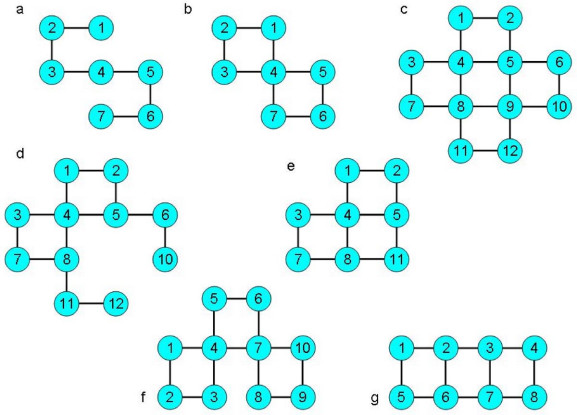
\includegraphics[width=0.9\linewidth]{Images/2d_clusters_rep.jpg}
  \label{I2dclustersfig}
  \caption{Figure from \protect\cite{gerald2006efficient}, showing representative 2D cluster shapes. The vertices are qubits with integer indices, and the edges indicate entanglement connectivity between select neighbors.}
\end{figure}


A cluster state can be represented as a graph $G = (N,E)$, where the $n\in N$ is a qubit and $e\in E$ is the application of a Controlled-$Z$ ($C_z$) gate, where:

\[
C_z = 
\begin{pmatrix}
  1 & 0 & 0 & 0 \\
  0 & 1 & 0 & 0 \\
  0 & 0 & 1 & 0 \\
  0 & 0 & 0 & -1 \\
 \end{pmatrix}
\]

A \textit{linear} cluster state is one where $degree(n) \leq 2 \forall n \in N$.

\begin{gather*}
\Qcircuit @C=1em @R=1em{
  &\cluster{1}&\cluster{2}\qw&\cluster{3}\qw&\cluster{4}\qw 
}\\
{\footnotesize \text{4-Node Linear Cluster State}}%
\end{gather*}

A method to prepare such a cluster state is given in \cite{jorrand2005unifying}, consisting of ``cascading'' $C_z$ gates on $n$ qubits as follows:

% I have custom commands in here -- see preamble
\[
  \Qcircuit @C=1em @R=.5em @!R{
    \lstick{\ket{+}_1}&\ctrl{1}&\lzyLbl{1}&\qw      &\lzyLbl{2} &\qw     &\lzyLbl{3}&\qw\\
    \lstick{\ket{+}_2}&\gate{CZ}&\lzyLine  &\ctrl{1}&\lzyLine   &\qw     &\lzyLine  &\qw\\
    \lstick{\ket{+}_3}&\qw      &\lzyLine  &\gate{CZ}&\lzyLine  &\ctrl{1}&\lzyLine  &\qw\\
    \lstick{\ket{+}_4}&\qw      &\qw       &\qw      &\qw       &\gate{CZ}&\qw      &\qw
  }
\]

We can then analyze the state of the qubits at each of the dotted lines:

\begin{description}
\item[\bf \textit{1:}]
\vspace{1em}
{\small
  \begin{gather*}
  \left(\frac{\ket{0}_1\ket{+}_2+\ket{1}_1\ket{-}_2}{\sqrt2}\right)\ket{+}_{3}\ket{+}_{4}\\
  \equiv\left(\frac{\ket{+}_1\ket{0}_2+\ket{-}_1\ket{1}_2}{\sqrt2}\right)\ket{+}_{3}\ket{+}_{4}
  \end{gather*}
  }%
\item[\bf \textit{2:}] 
{\small
\begin{gather*}
\left(\frac{\ket{+}_1\ket{0}_2\ket{+}_{3}+\ket{-}_1\ket{1}_2\ket{-}_{3}}{\sqrt2}\right)\ket{+}_{4}\\
\equiv\left(\frac{\ket{0}_1\ket{+}_2+\ket{1}_1\ket{-}_2}{2}\ket{0}_{3}+\frac{\ket{0}_1\ket{-}_2+\ket{1}_1\ket{+}_2}{2}\ket{1}_{3}\right)\ket{+}_{4}
\end{gather*}
}%
\item[\bf \textit{3:}]
{\scriptsize
\begin{gather*}
  \left(\frac{\ket{+}_1\ket{0}_2\ket{+}_3+\ket{-}_1\ket{1}_2\ket{-}_3}{2}\right)\ket{0}_4\\
  +\left(\frac{\ket{+}_1\ket{0}_2\ket{-}_3+\ket{-}_1\ket{1}_2\ket{+}_3}{2}\right)\ket{1}_4\\
\equiv\frac{
  (\ket{+}_{1}\ket{0}_2+\ket{-}_{1}\ket{1}_2)\ket{0}_3\ket{+}_4 +
  (\ket{+}_{1}\ket{0}_2-\ket{-}_{1}\ket{1}_2)\ket{1}_3\ket{-}_4}{2}
\end{gather*}
}%
\end{description}


The action of the $C_z$ gate in the computational basis can be seen to be $\ket{x,y} \to (-1)^{xy}\ket{x,y}$. Cluster states of arbitrary shape and connectivity can similarly be prepared via the recursive use of the Hadamard gate and two-qubit fusion operations \cite{browne2005efficient,gerald2006efficient}. 


\subsection{Preparation of T-Shaped Cluster State}

A cluster state without the limitation on the degree of a node allows us to build \textit{nonlinear} cluster states:
%That vertical line bugged me
\newcommand{\vertLine}{\ar@{-}[]+<0em,-2.6em>;[d]+<0em,2.6em>}
\begin{gather*}
\Qcircuit @C=1em @R=1.3em{
\cluster{1}&\cluster{2}\vertLine\qw&\cluster{3}\qw\\
&\cluster{4}&
}\\
{\footnotesize \text{4-Node T-Shaped Cluster State}}%
\end{gather*}


The circuit creating this cluster state will look as follows:
%See preamble for command definitions
\[
  \Qcircuit @C=1em @R=.5em @!R{
    \lstick{\ket{+}_1}&\ctrl{1}&\qw &\qw     &\qw &\qw     &\lzyLbl{ }&\qw\\
    \lstick{\ket{+}_2}&\gate{CZ}&\qw&\ctrl{1}&\qw &\ctrl{2}&\lzyLine  &\qw\\
    \lstick{\ket{+}_3}&\qw      &\qw&\gate{CZ}&\qw&\qw     &\lzyLine  &\qw\\
    \lstick{\ket{+}_4}&\qw      &\qw&\qw      &\qw&\gate{CZ}&\qw      &\qw
  }
\]

The state of the qubits after the application of the first two $C_z$ gates is identical to the linear case, and the state after the last $C_z$ (at the dotted line) is given by:

{
\begin{gather*}
  \frac{\ket{+}_1\ket{0}_2\ket{+}_{3}\ket{+}_4+\ket{-}_1\ket{1}_2\ket{-}_{3}\ket{-}_4}{\sqrt{2}}\\
  \equiv \frac{1}{\sqrt{2}}\left[\left(\frac{\ket{+}_1\ket{0}_2\ket{+}_3 + \ket{-}_1\ket{1}_2\ket{-}_3}{\sqrt{2}}\right)\ket{0}_4\right.\\
    \left.+\left(\frac{\ket{+}_1\ket{0}_2\ket{+}_3 - \ket{-}_1\ket{1}_2\ket{-}_3}{\sqrt{2}}\right)\ket{1}_4\right]
\end{gather*}
}%

It is important to emphasize that the order in which the $C_z$ gates are applied to grow the cluster state is irrelevant, as all of these pair-wise operations commute. This feature will be exploited later when discussing parallelizability.

\section{The Effects of Measurement on a Cluster State}

As is clear from the form of the expressions of all cluster states
illustrated thus far, measuring any node in the computational basis
severs it from the remaining graph by cutting all of it's edges with
it's neighboring nodes. Should the outcome of said measurement be $1$,
then a $Z$ gate/transform gets applied to all of it's erstwhile
neighbors in the leftover cluster state. Thus, a large cluster state
can be arbitrarily trimmed, split, and/or reshaped by removing qubits
from the cluster. This is accomplished by measuring the target qubit
in the computational basis, and performing appropriate unitary
rotations on its former neighbors based on the measurement outcome.

The effect of an $X$-measurement (\ie a computational basis measurement following a Hadamard transformation) on any node of the cluster state is much more involved. This is best illustrated when demonstrating the use of a linear cluster state as a wire for quantum information. For this exercise, we start with a linear cluster state with three nodes (labelled $1$, $2$, and $3$). A single qubit of quantum information $\ket{\psi} = \alpha\ket{0}+\beta\ket{1}$ is stored in a physical qubit labelled $0$ as illustrated below.

\begin{gather*}
  \Qcircuit @C=1em @R=1em{
    &\ket{\psi}_0&&&\\
    &\cluster{0}&\cluster{1}&\cluster{2}\qw&\cluster{3}\qw
    \gategroup{1}{2}{2}{3}{1.5em}{--}
}\\
{\footnotesize \text{Gate $C_z^{(0,1)}$, followed by measurements $M_X^{(0)}$, $M_X^{(1)}$, \& $M_X^{(2)}$.}}%
\end{gather*}

To teleport the state $\ket{\psi}$ to physical qubit number $3$, we must first supply the quantum information to the ``wire.'' This is achieved by applying a $C_z$ gate between physical qubits $0$ and $1$. Using $\ket{\mathcal{LC}}_{123}$ to denote the linear cluster state, we have

{
  \begin{gather*}
    C_z^{(0,1)}\ket{\psi}_0\otimes\ket{\mathcal{LC}}_{123} \\
    = \frac{1}{\sqrt{2}}[\alpha\ket{0}_0\ket{+}_1\ket{0}_2\ket{+}_3+\beta\ket{1}_0\ket{-}_1\ket{0}_2\ket{+}_3\\
      \alpha\ket{0}_0\ket{-}_1\ket{1}_2\ket{-}_3+\beta\ket{1}_0\ket{+}_1\ket{1}_2\ket{-}_3]
  \end{gather*}
}%

Following this, we perform $X$-measurements on physical qubits $0$, $1$, and $2$ in that order. Let us denote an $X$-measurement operation on the $j^{th}$-node with $M_X^{(j)}$, and let the outcome of any measurement on the same node be $m_j$. Then, the end result of these operations is the state

\begin{equation*}
  X^{m_2}Z^{m_1}X^{m_0}H\ket{\psi}_3,\quad\quad m_j\in\{0,1\}.
\end{equation*}

The quantum information $\ket{\psi}$ has successfully been teleported to physical qubit $3$, up to application of Pauli operators depending on the measurement outcomes. Since the leftover/extra Pauli operators do not commute, these measurements had to have been carried out in a specific order. However, the operation $C_z^{(2,3)}$, which was employed to grow the linear cluster state, commutes with $C_z^{(0,1)}$, as well as measurements $M_X^{(0/1)}$. Thus, further links to the chain can be grown as earlier links are being subjected to measurements. This aids in parallelizability, as well as physical implementation of cluster state quantum computing schemes.

Briegel and Raussendorf show that any quantum logic circuit can be implemented on a cluster state, which demonstrates universality of the proposed scheme \cite{briegel2000measurements}. Nielsen \cite{nielsen108020universal} extended this result to no longer require coherent dynamics, instead relying on a method to teleport quantum gates, and he provided a concise algorithm to accomplish this. 

\section{One-Way Quantum Computation}
All quantum computation schemes may be characterized by some combination of state preparation, unitary transformation of said states, and measurements on the same. Human-usable computational tasks necessarily require both input and final output to be classical information. The classical input information can influence the quantum computation in choice of initial states, the choice of unitary transforms (\ie algorithm), and the choice of measurement bases. The output is always a classical function of the measurement outcomes. In typical models for quantum computation, entire algorithms are implemented as a sequence of unitary transformations on a prepared quantum state (stored in qubits) of size appropriate to the problem, with a round of measurements as the final step. In such models, the unitary transformation stage is completely reversible. The splitting of the effective unitary matrix into sequential steps can be arbitrary and entirely dependent on physical hardware limitations. There is no correspondence with ``computational steps'' or ``clock cycles'' in the classical sense, as the quantum state of the computer in the midst of the unitary stages is inaccessible for diagnosis or debugging purposes. Any leakage of information into computer memory or environment constitutes decoherence, and will introduce errors in the computation.


One-way quantum computation, on the other hand, revolves around single qubit measurements as a progression of computational steps. Measurements are a crucial component to quantum information processing because they irreversibly destroy a quantum state. Entanglement, on the other hand, will ensure that the state of the final qubit relies on the outcomes of preceding measurements. Given a cluster state, a series one-qubit measurements can be performed at each qubit to implement a quantum gate \cite{jorrand2005unifying}.  The unidirectionality of cluster state computation is inherent, due to the fact that quantum information cannot be accurately recovered once a measurement has been made. Consider a two-dimensional array of entangled qubits, information propagates horizontally through a row of qubits while vertical qubit neighbors are used for two-qubit gates. Similarly, three-dimensional clusters can be used to implement topologically protected gates \cite{raussendorf2007topological}, where the gate function only depends upon the way ``connected defects'' are wound around one another, but not on the details of their shape. This degree of freedom affords the design some fault tolerance.


The basic principle of cluster-state quantum computation is to effectively enact arbitrary quantum circuits onto qubits storing quantum information by performing single-qubit transformations and measurements on a pre-formed cluster state whose graph representation bears topological similarities to the circuit in question. These measurements result in destruction of the node-qubits of the cluster state, and hence are irreversible. The outcomes of these measurements need to be tracked or fed forward to influence future operations along certain layers of the cluster, as will be illustrated later in this article.


\begin{gather*}
 \Qcircuit @C=1em @R=1.2em {
   & \gate{A} & \multigate{1}{C} & \qw & \gate{E} & \multigate{2}{G} & \multigate{1}{J} & \qw \\
   & \gate{B} & \ghost{C} & \gate{D}  & \multigate{1}{F} & \ghost{G} & \ghost{J} & \qw \\
   & \qw & \qw & \qw & \ghost{F} & \ghost{G} & \gate{K} & \qw \\
 }\\
 {\footnotesize \text{Arbitrary quantum circuit involving unitary operations on 3 qubits.}}%
 \end{gather*}

 \newcommand{\certLine}{\ar@{-}[]+<0em,-1.em>;[d]+<0em,1.em>}
 \begin{gather*}
 \Qcircuit @C=0.5em @R=0.5em{
    &\cluster{}\qw&\qw&\cluster{}\certLine\qw&\qw&\qw&\qw&\cluster{}\qw&\qw&\cluster{}\certLine\qw&\qw&\cluster{}\certLine\qw&\qw&\cluster{}\certLine\qw&\qw\\
   &\cluster{}\qw&\qw&\cluster{}\qw&\qw&\cluster{}\qw&\qw&\cluster{}\certLine\qw&\qw&\cluster{}\certLine\qw&\qw&\cluster{}\certLine\qw&\qw&\cluster{}\qw&\qw\\
    &\qw&\qw&\qw&\qw&\qw&\qw&\cluster{}\qw&\qw&\cluster{}\qw&\qw&\cluster{}\qw&\qw&\cluster{}\qw&\qw\\   
 }\\
           {\footnotesize \text{Single-qubit measurements on this cluster state is equivalent}}\\
            {\footnotesize \text{to the topologically similar circuit above.}}%
 \end{gather*}

\subsection{Gates through teleportation}
%\clr Xiaodi mentioned that gate application via teleportation was the motivation for cluster states to begin with. This is basically Maira's segment of the talk. Can she turn it into motivational prose? No she cannot. Writing is not her forte. 
Quantum teleportation is a procedure by which quantum information can be transferred from one point to another via two classical bits of information if the sender and received previously shared an entangled state. It is useful for quantum computation however, this approach uses an entangled state as a resource but if that state has some error then teleportation fails. Gottesman and Chuang \cite{gottesman1999demonstrating} first showed that if the entangled state $\ket{\psi}$ can be replaced by $U\ket{\psi}$, such that $U$ is a non-trivial quantum operation. The corresponding output $U\ket{\alpha}$ is in the initial state $\ket{\psi}$ but with additional single-qubit Pauli operations $X$, $Y$, or $Z$. By simply reversing the Pauli operators the original state can be reconstructed. This teleportation scheme can be useful in applying other gates that are non-trivial. 


\begin{gather*}
HZ_\alpha=\frac{1}{\sqrt2}\left(\begin{array}{cc}
e^{\frac{-i\alpha}{2}} & e^{\frac{i\alpha}{2}}\\
e^{\frac{-i\alpha}{2}} & -e^{\frac{i\alpha}{2}}\end{array}\right)
\end{gather*}

As demonstrated in the previous section, by applying single-qubit gates we can teleport one state from one side of a cluster state to the other. In this section we demonstrate how to apply the $HZ_\alpha$ gate through teleportation.
 
\begin{gather*}
\Qcircuit @C=1em@R=0.5em @!R{
\lstick{\ket{+}_1} & \ctrl{1} & \qw & \gate{ HZ_{\alpha 1} } & \meter   \\
 \lstick{\ket{+}_2} & \gate{CZ} & \ctrl{1}  & \qw & \gate{ HZ_{\pm \alpha 2} }\cwx & \meter \\
 \lstick{\ket{+}_3} & \qw & \gate{CZ}  & \qw & \qw & \qw
}
\end{gather*}


In this example we will apply two consecutive $HZ_\alpha$ gates to our cluster to simulate two gates on a single qubit. We will demonstrate that the outcome is the same except for an additional two Pauli operations. For this problem we prepare a three node cluster state given by: 
{
\begin{gather*}
C_{z}^{(1,2)}C_{z}^{(2,3)}\ket{+}_1\ket{+}_2\ket{+}_3 = \ket{\psi_1} \\
=\frac{1}{\sqrt2}\ket{0}_1\left(\ket{0}_2\ket{+}_3+\ket{1}_2\ket{-}_3\right)\\
+\frac{1}{\sqrt2}\ket{1}_1\left(\ket{0}_2\ket{+}_3-\ket{1}_2\ket{-}_3\right)
\end{gather*}
}%

First we will apply $HZ_{\alpha1}$ and measure in the computational basis. 
{
\begin{gather*}
HZ_{\alpha1}\ket{\psi_1}=\frac{e^{-i\alpha_{1}/2}}{2}\ket{+}_1\left(\frac{\ket{0}_2\ket{+}_3+\ket{1}_2\ket{-}_3}{\sqrt2}\right)\\
+\frac{e^{i\alpha_{1}/2}}{2}\ket{-}_1\left(\frac{\ket{0}_2\ket{+}_3-\ket{1}_2\ket{-}_3}{\sqrt2}\right)=\ket{\psi_2}
\end{gather*}
}%


For convenience we assume that we measure the state $\ket{0}$.

{
\begin{gather*}
X^{0}\ket{\psi_2}=\frac{1}{\sqrt2}\cos{(\alpha_1/2)}\ket{0}_2\ket{+}_3\\
-\frac{i}{\sqrt2}\sin{(\alpha_1/2)}\ket{1}_2\ket{3}_3=\ket{\psi_3}
\end{gather*}
}% 
\vspace{2ex}
We apply one final $HZ_{\alpha}$ gate. 
{
\begin{gather*}
HZ_{\pm\alpha2}\ket{\psi_{3}}=\ket{\psi_4}\\
\frac{1}{\sqrt2}\ket{0}_2\left(\cos{(\frac{\alpha_1}{2})}e^{-i\alpha_2/2}\ket{+}_3-i\sin{(\frac{\alpha_1}{2})}e^{i\alpha_2/2}\ket{-}_3\right)\\
+\frac{1}{\sqrt2}\ket{1}_2\left(\cos{(\frac{\alpha_1}{2})}e^{-i\alpha_2/2}\ket{+}_3+i\sin{(\frac{\alpha_1}{2})}e^{i\alpha_2/2}\ket{-}_3\right)
\end{gather*}
}%

The final output state we get is:

{
\begin{gather*}
X^{0}\ket{\psi_{4}}=\ket{\psi_5}=\frac{1}{\sqrt2}\cos{(\frac{\alpha_1}{2})}e^{-i\alpha_2/2}\ket{+}_3\\
-\frac{i}{\sqrt2}\sin{(\frac{\alpha_1}{2})}e^{i\alpha_2/2}\ket{-}_3
\end{gather*}
}%

 The output of the circuit is $X^{m_2}HZ_{\pm\alpha2}X^{m_1}HZ_{\alpha1}\ket{+}_3$, where $m_1$ and $m_2$ are the outputs for the first and second qubits. Analyzing this output a bit further we see that $HX^{m_1}=Z^{m_1}H$ and $Z_{\pm\alpha2}X^{m_1}=X^{m1}Z_{\alpha2}$. Using this the state can be rewritten as:
\begin{gather*}
X^{m_2}Z^{m_1}HZ_{\alpha2}HZ_{\alpha1}\ket{+}_3
\end{gather*}

This is equivalent to the output of the conventional single-qubit quantum circuit up to a known Pauli matrix. Thus it is easy to model gate application through teleportation.

We observe that in the circuit given below the two highlighted boxes are both one-bit teleportations. Because the $C_z$ gate commutes with $HZ_\alpha$ we can perform one teleportation procedure and then the second one or vice-versa. This is advantageous because it means that we can build the cluster as we go.


\begin{gather*}
\Qcircuit @C=1em @R=1em{
&\lstick{\ket{+}_1} &\ctrl{1} & \gate{HZ_{\alpha1}} & \meter & \cw & \cw \\
&\lstick{\ket{+}_2} & \gate{CZ} & \qw & \qw & \ctrl{1} & \gate{HZ_{\pm\alpha2}} \cwx  & \meter \\
&\lstick{\ket{+}_3} & \qw & \qw & \qw & \gate{CZ} & \qw & \qw \gategroup{1}{5}{2}{3}{0.8em}{--} \gategroup{2}{6}{3}{8}{1.2em}{--}
}
\end{gather*}



\clbl

\clbl
\subsection{Applying a 2-qubit gate via 2D cluster state}

The ability to implement gates of the form $HZ_\alpha$, and any 2-qubit controlled-phase gate, and to prepare arrays of $\ket{+}$ states as inputs, constitute a set of resources that is universal for quantum computation \cite{jozsa2006introduction}. In this subsection, we will demonstrate the use of two-dimensional cluster states to implement a $C_z$ gate between two input kets bearing quantum information $\ket{\phi_A}_A\ket{\phi_B}_B$ encoded in physical qubits labelled `A' and `B.' Here, $\ket{\phi_j} := \alpha_j\ket{0}+\beta_j\ket{1}$. For the scheme, we will use an I-shaped cluster states with six nodes, as shown in the figure. 

\newcommand{\bertLine}{\ar@{-}[]+<0em,-2.3em>;[d]+<0em,2.3em>}
\begin{gather*}
  \Qcircuit @C=1em @R=1em{
    \ket{\phi_A}&\cluster{\Scale[0.8] A}&\cluster{1}&\qw&\cluster{2}\bertLine\qw&\qw&\cluster{3}\qw\\
    \ket{\phi_B}&\cluster{\Scale[0.8] B}&\cluster{5}&\qw&\cluster{4}\qw&\qw&\cluster{6}\qw
    \gategroup{1}{1}{2}{3}{2.2em}{--}
}\\
{\footnotesize \text{Apply $C_z^{(A,1)}$ and $C_z^{(B,5)}$ to input quantum information into cluster state.}}%
\end{gather*}

The procedure would be to first entangle the input quantum information qubits into the cluster state via the application of $C_z$ gates. Then we perform single qubit measurements on all qubits but numbers $3$ and $6$. Using the $Z$-measurement property of nodes on cluster states, we can pick node $4$ as a representative anchor and write down the total state of the current system as

\begin{gather*}
  \frac{1}{\sqrt{2}}\left[\ket{\mathcal{LC}}_{123}\ket{0}_4\ket{+}_5\ket{+}_6+Z_{2}\ket{\mathcal{LC}}_{123}\ket{0}_4\ket{-}_5\ket{-}_6\right]\\\otimes\ket{\phi_A}_A\ket{\phi_B}_B,
\end{gather*}

\noindent where $Z_{2}$ is being applied on qubit $2$.

The single qubit mesurements have to be performed in the order ($M^{(A)}_X, M^{(1)}_X, M^{(2)}_X$) and ($M^{(B)}_X, M^{(5)}_B, M^{(4)}_X$). These two subsets are parallelizable, and one could perform the measurements \{$M^{(A)}_X, M^{(B)}_X$\} in parallel, and then \{$M^{(1)}_X, M^{(5)}_X$\}, and so on. But here, we will introduce the concept of layers of measurement, by performing all bottom row operations at once (including input entanglement), and then working on the top row.

Enacting the gate $C_z^{(B,5)}$ on the initial state, followed by measurements $M^{(B)}_X, M^{(5)}_B, M^{(4)}_X$ yields random outcomes $m_B, m_5, m_4 \in \{0,1\}$ and  gives us the state

\begin{gather*}
  X_6^{m_4}Z_6^{m_5}X_6^{m_B}C_Z^{(2,6)}\ket{\mathcal{LC}}_{123}\ket{\phi_B}_6\otimes\ket{\phi_A}_A.
\end{gather*}

Note that even though the original cluster state had an edge between nodes $2$ and $4$ in the graph representation, a measurement on qubit $4$ did not sever the link between node $6$ and the linear chain $\ket{\mathcal{LC}}_{123}$, due to the measurements being in the $X$ basis. Now, if we follow the above operations by application of the $C_Z^{(A,1)}$ gate, and the measurements $M^{(A)}_X, M^{(1)}_X, M^{(2)}_X$ in that order, we get the random results $m_A, m_1, m_2 \in \{0,1\}$ and the final state

\begin{gather*}
  X_3^{m_2}Z_3^{m_1}X_3^{m_A}H_3X_6^{m_4}Z_6^{m_5}X_6^{m_B}H_6C_X^{(6,3)}\ket{\phi_A}_3\ket{\phi_B}_6,
\end{gather*}

\noindent where $C_X^{(j,k)}$ is the controlled-NOT gate. All single-qubit operations on qubit $3$ commute with single-qubit operations on qubit $6$. Using the fact that $H_j^2 = I_j$, as well as $C_X^{(6,3)}\equiv (H_3\otimes I_6)C_Z^{(3,6)}(H_3\otimes I_6)$, the final state is equivalently

\begin{gather*}
  X_3^{m_2}X_6^{m_4}Z_3^{m_1}Z_6^{m_5}X_3^{m_A}X_6^{m_4}H_6C_Z^{(3,6)}H_3\ket{\phi_A}_3\ket{\phi_B}_6,
\end{gather*}

\noindent which is the desired result, up to overall Pauli transformations on the individual qubits. Thus, we have proven that a universal set of quantum operations can be implemented using the cluster state model.

\subsection{Commutations and parallelizability}

The previous subsections demostrated that although measurements in a
specific layer (an ordered set of sequentially connected nodes) of a
cluster state need to occur in a specific order, operations on
different layers commute, and can therefore be interspersed. This,
combined with the ability to delay the growth of the cluster state to
occur just before the measurements catch up with the remaining nodes,
offers several possibilities for process parallelization.

\begin{figure}[thb]
  \centering
  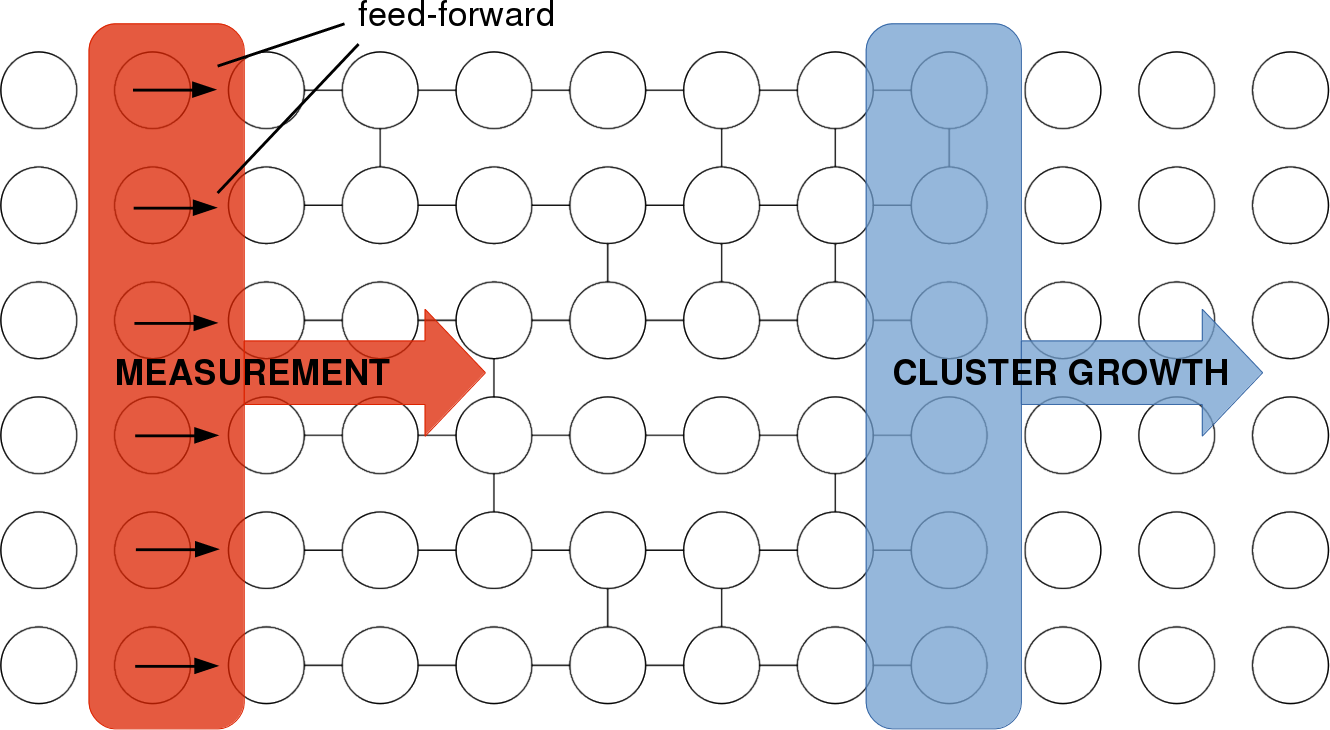
\includegraphics[width=\linewidth]{Images/parallel01.png}
  \label{parallelfig1}
  \caption{The controlled-phase operations commute with unitaries and measurements on other parts of the cluster state. This allows one to conserve and reuse physical resourses, as well as maintain coherence on smaller cluster sizes at any given time.}
\end{figure}


Indeed, in the $2$-qubit gate example, the quantum information in one of the qubits was put into the system first, followed by some measurement-based teleporation, and the other input qubit was brought in later. We effectively managed to entangle the two qubits using only single-qubit measurements.

\begin{figure}[hbt]
  \centering
  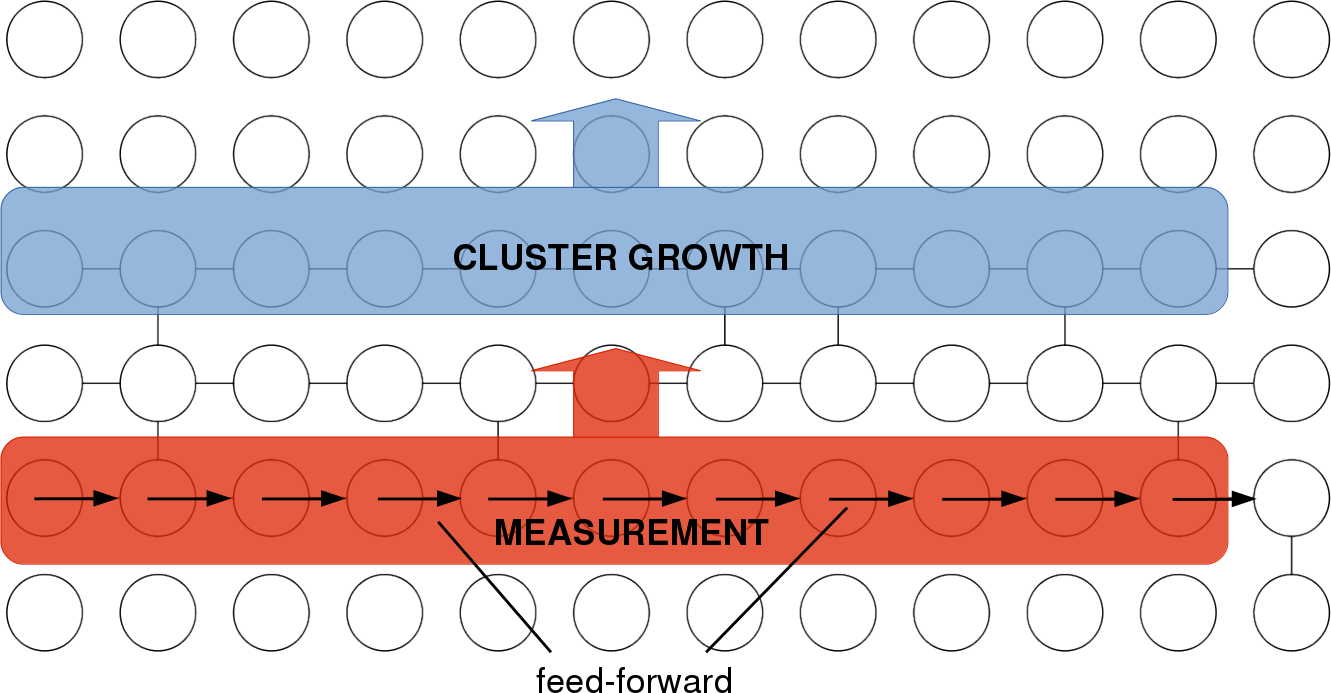
\includegraphics[width=\linewidth]{Images/parallel02.png}
  \label{parallelfig2}
  \caption{X-measurements do not sever ``vertical'' links despite destruction of qubits. This allows different linear layers to be processed in any order.}
\end{figure}

This seems to indicate that all multi-qubit interactions can be pre-computed by setting the topological layout of the graph of the cluster state before any of the quantum information has even been introduced into the system. 

%\section{Gate Array Correspondence}
%In his analysis of the reducibility of 1WQC to the gate array model, Richard Jozsa gives a polynomial time algorithm to perform the conversion between the two computational models \cite{jozsa2006introduction}. 
%>>>>>>> Stashed changes

\begin{figure*}[t]
  \centering
  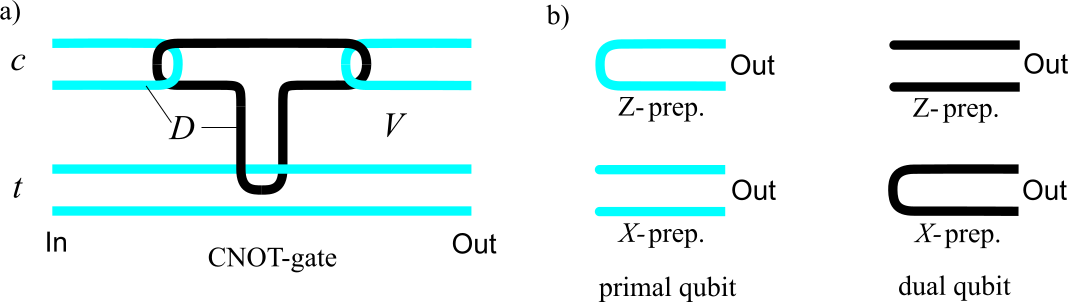
\includegraphics[width=0.7\linewidth]{Images/topological01.png}
  \caption{Figure from \protect\cite{goyal2007}. Topologically protected gates as realized in three-dimensional cluster states. (a) An individual encoded CNOT gate with control $c$ and target $t$. (b) The preparation of logical qubits in the \{$\ket{0}$, $\ket{1}$\} (\ie $Z$-) and the \{$\ket{\pm}$\} (\ie $X$-) bases. The line-like structures are connected defect sites (nodes measured in the $Z$-basis, denoted by set `D') embedded in a 3D lattice, surrounded by sites belonging to set `V' (measured in the $X$-basis). The gate function only depends upon the way the defect lines are wound around one another.}
  \label{topologicalfig1}
  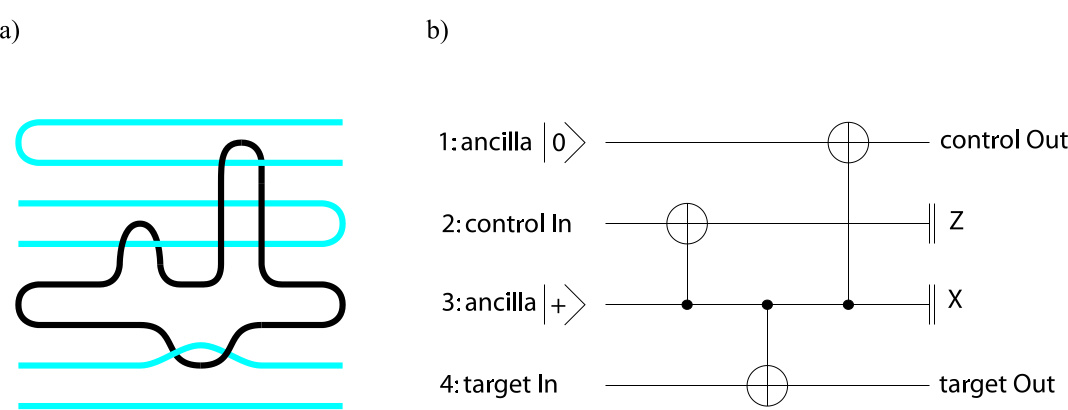
\includegraphics[width=0.7\linewidth]{Images/topological02.png}
  \caption{Figure from \protect\cite{goyal2007}. (a) Another version of the CNOT gate topologically equivalent to that shown in figure \ref{topologicalfig1}(a). (b) Equivalent circuit, representing a CNOT gate between the control and target qubit.}
  \label{topologicalfig2}  
\end{figure*}

\subsection{3D cluster states and topological fault tolerance}

While 2D cluster states are sufficient for fully realizing any quantum computation, Goyal et al \cite{goyal2007} have exploited a correspondence between quantum gates, quantum correlations, and surfaces to propose a topological model for cluster-state quantum computation. The method affords them a (fault-tolerance) threshold estimate of $0.75$\% for each source in an error model with preparation, gate, storage and measurement errors, with a poly-logarithmic multiplicative overhead in the circuit size. While a full detailed description of this approach is beyond the scope of this article, here we present a brief overview.

In their scheme, a 3D cluster state consisting of a lattice of qubits is `carved out' with 1D line-like defects via $Z$-measurements on connected physical qubits. This results in a nontrivial cluster topology in which a fault-tolerant quantum circuit is embedded (figure \ref{topologicalfig1}). These line defects essentially simulate anyons \cite{sarma2008}, and the way they knot and loop around each other effectively obeys non-Abelian braiding statistics, allowing one to simulate gates (figure \ref{topologicalfig2}). The fault tolerance comes from the topological invariance of the structures to local perturbations to the line defects (such as specific path and length). One of the dimensions of this 3D representation can be mapped to `simulated time,' which is a necessary facet of all computation that maps inputs to outputs. This mapping can be literal in physical 2D cluster states.

\section{Computational Power and Complexity}
The spacial layout of the graph representation of the cluster state plays a role in the computational power of that state. If a cluster state can be prepared linearly via the cascading $C_z$ technique mentioned above, it can be represented as a  ``one-dimensional'' graph (i.e., some graph $G=(V,E),\ \forall v\in V$, deg$(v)\leq 2$). Operations on a linearly prepared cluster state can be efficiently simulated on a classical computer in $O(n\log ^c (1/n))$, where $n$ is the initial number of qubits, and $c$ is the cost of floating point multiplication \cite{nielsen2006cluster}. Though the author consequently dismisses linearly prepared cluster states as a substrate for quantum computation, it would be interesting to know which class of problems they would be able to solve.

\subsection{Gate Array Reductions}


With only a bit of construction, it can be seen that the cluster state model is polynomially reducible to the gate array model, and the converse is also true. To see this, we first need to create a definition of the standard gate array model:

\vspace{1em}
\begin{enumerate}
\item All measurements take place at the end of the circuit
\item All measurements take place in the computational basis
\end{enumerate}

\vspace{1em}
We can now generalize this definition to allow measurements along the way with subsequent choices of gates and measurements being allowed to depend on earlier measurement outcomes. Intuitively, what we will do is add an ancilla bit to all measurements which take place before the end, and perform controlled operations with this ancilla to return to the standard definition. Specifically, for all measurements in the $\{ U\ket{0}, U\ket{1} \}$ basis, we add an ancillary qubit $A$, (initially in state $\ket{0}$) and replace the measurement with an application of $U^\dagger$ to $B$ followed by applying $C_X$ to $BA$ as shown:

\begin{figure}[H]
  \begin{gather*}
  \Qcircuit @C=1em @R=1em{
  &\lstick{B} & \qw & \meter & \cw & \cw 
  }
  \end{gather*}
  \caption{Some non-standard circuit}

  \begin{gather*}
  \Qcircuit @C=1em @R=1em{
  &\lstick{B}       & \gate{U^\dagger} & \ctrl{1} & \qw \\
  &\lstick{\ket{0}} & \qw              & \gate{X} & \qw
  }
  \end{gather*}
  \caption{An equivalent standard circuit}
\end{figure}


Now, any future gates that depended on the measurement outcome are replaced by a corresponding controlled operation, controlled by the state of $A$. It is therefore clear that this process converts any non-standard circuit to the standard gate array model.

\subsubsection{Reducing Cluster State to Gate Array}
The above technique shows how a cluster state circuit is converted into an equivalent (standard) gate array. In addition to building the required cluster state using an array of $C_Z$ gates acting on $\ket{+}$ states, we introduce an ancilla $A$ for each 1-qubit measurement. For each $M(\theta)$ measurement we introduce an extra gate $W^\dagger (\theta)$ which transforms the $M(\theta)$ basis to the standard basis. 

\begin{figure}[H]
  \begin{gather*}
  \Qcircuit @C=1em @R=1em{
  &\lstick{\ket{+}} & \ctrl{1} & \gate{M(\theta)} & \cw & \cw \\
  &\lstick{\ket{+}} & \gate{Z} & \qw
  }
  \end{gather*}
  \caption{A two qubit cluster state}

  \begin{gather*}
  \Qcircuit @C=1em @R=1em{
  &                 &          & \lstick{\ket{0}} & \gate{X} & \qw \\
  &\lstick{\ket{+}} & \ctrl{1} & \gate{W^\dagger (\theta)} & \ctrl{-1}& \qw \\
  &\lstick{\ket{+}} & \gate{Z} & \qw              & \qw      & \qw
  }
  \end{gather*}
  \caption{An equivalent cluster state with ancilla}
\end{figure}


Thus, to convert the measurement-based cluster state model to the gate array model requires polynomially more gates and qubits (one per measurement).


\subsubsection{Reducing Gate Array to Cluster State}
To see how an arbitrary gate array can be converted to the cluster state model, we first need some universal gate set $G$ (for information on what this set might contain, see \cite{shi2002both}). For each gate within this set, we can specify some number which represents the number of measurements that a 1WQC would have to perform to get the same outcome. These numbers can then be used to partially order a set, allowing us to pick $K$, which represents the maximum number of measurements required to simulate any single gate from the set. From this, we can see that even if some circuit contained only this ``most expensive'' gate, the number of additional qubits and gates would be a factor of $K$ (polynomial).


\subsection{Quantum Layers}
The above reduction strategy provides a nice way of categorizing a given quantum algorithm into its classical and quantum parts:

\begin{itemize}
\item The classical parts are those that are done serially (i.e. the decision of future gates based on measurement outcomes)
\item The quantum parts are those that can be done in parallel
\end{itemize}

From this, we can see that the cluster state model exemplifies both parts, but the gate array model only does ``quantum parts''. With this idea, we can define the notion of layers by saying that a quantum process with $K$ layers is one where $K$ gates are operating in parallel. The above suggests the following conjecture \cite{jozsa2006introduction}:

\begin{description}
\item[Conjecture:] Any polynomial time quantum algorithm can be implemented with only $O(\log n)$ quantum layers interspersed with polynomial time classical computations.
\end{description}


This conjecture remains unproven in general, but it has been shown to hold for Shor's algorithm \cite{cleve2000fast}.


\subsection{Cluster graphs as an analysis tool}

Outside of the physical implementation considerations, cluster state model isomorphisms offer a new analysis tool that disentangles the quintessential influence of quantum formalism on the complexity class of various algorithms.

We have already shown in section IV, how any quantum algorithm that is expressible via a quantum gate-array circuit can equivalently be computed via single-qubit operations and measurements on a cluster state represented by a graph whose connectivity is topologically similar to the circuit diagram. This equivalence is purely geometric and is independent of the specific gates being applied (those are determined by the choice of measurements on the cluster state). This allows us to reduce entire classes of algorithms to specific types of graphs with designated input and output nodes for state-preparation and final-result measurements. We conjecture that the size of this graph has a bearing on the computational time of the entire class of algorithms. Furthermore, the multi-dimensional connectivity of said graphs embodies entangling operations, and serves to explicitly quantify any gains in complexity quantum offers over classical methods. And finally, the connectivity and feed-forward paths allows one to define modular operations that are independent of each other, and can help exploit all avenues for parallelization more effectively.

\section{Physical implementations}

Although the chief inspiration for cluster-state quantum computation was the ability to enact gates via teleportation, another motivation proved to be the extant experimental realizations of material qubits arranged in 2D arrays in physical space; be they cold atoms in optical lattices \cite{bloch2003}, or 2D ion traps \cite{rabchuk2006}, or other stationary qubits embedded in material substrates (quantum dots, superconducting qubits). The geometry of such systems encourages designs involving programming a quantum circuit into the device by literally ``etching'' the circuit diagram onto the 2D qubit array.

\subsection{Cluster states can't be ground states of Hamiltonians}



\subsection{Two qubit operations on non-photonic matter qubits}

\subsection{Nondeterministic two-qubit gates with linear optics}

\cite{klm2000}.

\subsection{Continuous-variable cluster states}


\section{Conclusions and Acknowledgements}

%To pad this out to ten pages, we can work on physical systems, limitations of linear optics, 3D fault tolerant model, and complexity theory. If we REALLY have time, there may or may not be something to be done with qudits.

%This is the stuff to work into the midterm
% \section{Proposal}

% This project will attempt to discuss background on cluster states, a correspondence between 1WQC and the more traditional gate array model, and the computational power of this new model. A primary goal is to review the literature surrounding 1WQCs and cluster states to motivate measurement-only based quantum computation. The concept will be presented as an extension of basic quantum teleportation. By the midterm report we hope to discuss in detail the various proposed qubit systems, including photonic, flux, and charge qubits, and cavity input-output theory for cluster state generation.  Additionally, the report will outline how to implement any quantum logic network onto a 1WQC with an easy example. 

% The final paper will focus on the complexity and universality of this model and explore the physical implementations of cluster states, with special emphasis on optics related technologies. We will illustrate possible advantages and disadvantages cluster states have in contrast to other approaches. If time permits, we also intend to explore fault-tolerant cluster state schemes, and the implications of cluster states with qudits.


%% file citations.bib contains all the bibliography
\bibliography{citations}
\end{document}
